% Copyright (C) 2021-2022 Diogo Rodrigues
% Distributed under the terms of license
% Creative Commons Attribution-NonCommercial-NoDerivatives 4.0 International

\documentclass[dvipsnames]{beamer}
% Encodings (to render letters with diacritics and special characters)
\usepackage[utf8]{inputenc}
% Language
\usepackage[english]{babel}
\usepackage{verbatim}

\usepackage{multicol}

\usepackage{setspace}

\usetheme{Madrid}
\usecolortheme{default}

\pdfstringdefDisableCommands{
  \def\\{}
  \def\texttt#1{<#1>}
}

\newcommand{\email}[1]{{\footnotesize\texttt{\href{mailto:#1}{#1}}}}

\usepackage{caption}
\DeclareCaptionFont{black}{\color{black}}
% \DeclareCaptionFormat{listing}{{\tiny \textbf{#1}#2#3}}
% \captionsetup[lstlisting]{format=listing,labelfont=black,textfont=black}
\usepackage{subfigure}

\usepackage{listings}
\lstset{
    % frame=tb, % draw frame at top and bottom of the code
    basewidth  = {0.5em,0.5em},
    % numbers=left, % display line numbers on the left
    showstringspaces=false, % don't mark spaces in strings  
    commentstyle=\color{PineGreen}, % comment color
    keywordstyle=\color{blue}, % keyword color
    stringstyle=\color{red}, % string color
	  aboveskip=0.5em,
    belowskip=0.5em,
    basicstyle=\scriptsize\ttfamily
}
\lstset{literate=
  {á}{{\'a}}1 {é}{{\'e}}1 {í}{{\'i}}1 {ó}{{\'o}}1 {ú}{{\'u}}1
  {Á}{{\'A}}1 {É}{{\'E}}1 {Í}{{\'I}}1 {Ó}{{\'O}}1 {Ú}{{\'U}}1
  {à}{{\`a}}1 {è}{{\`e}}1 {ì}{{\`i}}1 {ò}{{\`o}}1 {ù}{{\`u}}1
  {À}{{\`A}}1 {È}{{\'E}}1 {Ì}{{\`I}}1 {Ò}{{\`O}}1 {Ù}{{\`U}}1
  {ä}{{\"a}}1 {ë}{{\"e}}1 {ï}{{\"i}}1 {ö}{{\"o}}1 {ü}{{\"u}}1
  {Ä}{{\"A}}1 {Ë}{{\"E}}1 {Ï}{{\"I}}1 {Ö}{{\"O}}1 {Ü}{{\"U}}1
  {â}{{\^a}}1 {ê}{{\^e}}1 {î}{{\^i}}1 {ô}{{\^o}}1 {û}{{\^u}}1
  {Â}{{\^A}}1 {Ê}{{\^E}}1 {Î}{{\^I}}1 {Ô}{{\^O}}1 {Û}{{\^U}}1
  {Ã}{{\~A}}1 {ã}{{\~a}}1 {Õ}{{\~O}}1 {õ}{{\~o}}1
  {œ}{{\oe}}1 {Œ}{{\OE}}1 {æ}{{\ae}}1 {Æ}{{\AE}}1 {ß}{{\ss}}1
  {ű}{{\H{u}}}1 {Ű}{{\H{U}}}1 {ő}{{\H{o}}}1 {Ő}{{\H{O}}}1
  {ç}{{\c c}}1 {Ç}{{\c C}}1 {ø}{{\o}}1 {å}{{\r a}}1 {Å}{{\r A}}1
  {€}{{\euro}}1 {£}{{\pounds}}1 {«}{{\guillemotleft}}1
  {»}{{\guillemotright}}1 {ñ}{{\~n}}1 {Ñ}{{\~N}}1 {¿}{{?`}}1
}

\usepackage{dirtree}

\usepackage[style=british]{csquotes}

\usepackage{tabularx}

\usepackage{tikz}


\usepackage{svg}
\usepackage{graphicx}
 
%Information to be included in the title page:
\AtBeginDocument{
\title[\#1. Git Flow]{Git Flow}
\subtitle[]{Monitor session \#1}
\author[Diogo Rodrigues]{
  Diogo Miguel Ferreira Rodrigues (\email{diogo.rodrigues@fe.up.pt})
}
\institute[FEUP/LBAW]{Faculty of Engineering of the University of Porto \\ Database and Web Applications Laboratory (LBAW)}
\date[10/11/2021]{10th of November, 2021}
}

\begin{document}
\frame{\titlepage}

\begin{frame}
\frametitle{1. Some concepts}
\framesubtitle{1.1. What is git?}

\begin{minipage}{0.49\textwidth}
  Git is a version control program.
  
  \begin{itemize}
    \item Track changes in a set of files (a \textit{repository}, or just \textit{repo})
    \item Collaborate with other people
  \end{itemize}

\end{minipage}%
\begin{minipage}{0.51\textwidth}
  \centering
  \includesvg[width=40mm]{img/git-logo}
\end{minipage}

\vspace{2em}

Main points:

\begin{itemize}
  \item It is just a program in your computer
  \item There is {\footnotesize (almost)} \textbf{no Internet} in the way git works
\end{itemize}

Git contains your whole repository, including past versions.

\end{frame}

\begin{frame}
\frametitle{1. Some concepts}
\framesubtitle{1.2. What is GitHub/GitLab?}

GitHub/GitLab are companies that remotely host git repositories.

{\footnotesize (\textit{Really? Just that?} Basically yes, although they provide some extra services) }

\vspace{0.5em}

\vspace{1em}

\begin{minipage}{0.60\textwidth}
  \begin{itemize}
    \item Simplest and most common way to make git distributed and collaborative
    \item Each remote repository is accessible through a link (\textit{origin})
    \item To contribute to a repo:
    \begin{enumerate}
      \item Clone 
\includegraphics[height=3mm]{img/upload-download}
      \item Edit
      \item Commit
      \item Push 
\includegraphics[height=3mm]{img/upload-download}
    \end{enumerate}
  \end{itemize}
\end{minipage}%
\begin{minipage}{0.40\textwidth}
  \centering
  
\includegraphics[width=15mm]{img/GitHub-logo}\hspace{0.5em}
  \includesvg[width=15mm]{img/GitLab-logo}
\end{minipage}

\end{frame}

\begin{frame}
\frametitle{1. Some concepts}
\framesubtitle{1.3. Others}

\textbf{Tag:} human-readable name (an alias) for a particular commit.

\textbf{Wiki:} a special documentation zone to place everything that does not belong with the code.
The wiki is itself a git repo

\textbf{.gitignore:} special file containing file patterns that git should ignore (e.g., binary files)

\end{frame}

\begin{frame}
  \frametitle{2. Main subjects}
  \begin{center}
    \Large \textbf{Why use issues, branches, pull requests?}
  \end{center}

  \begin{itemize}
    \item Compile bugs, to-do functionalities (user stories), code reviews
    \item Interconnected with each other, and with references to code
    \item What has to do with code, stays near the code
    \item A chat is not enough: issues get mixed together and are not sufficiently clarified
  \end{itemize}

\end{frame}

\begin{frame}
  \frametitle{2. Main subjects}
  \framesubtitle{2.1. Issues}
  
  \footnotesize

  An issue is not necessarily a problem with the code, it is more like a \textit{to-do item} (e.g., "Fix list of users not showing", "Implement user page")

  
  
  \begin{center}
    \begin{tikzpicture}
      \tiny
      \node[inner sep=0pt] (img) at (0,0) {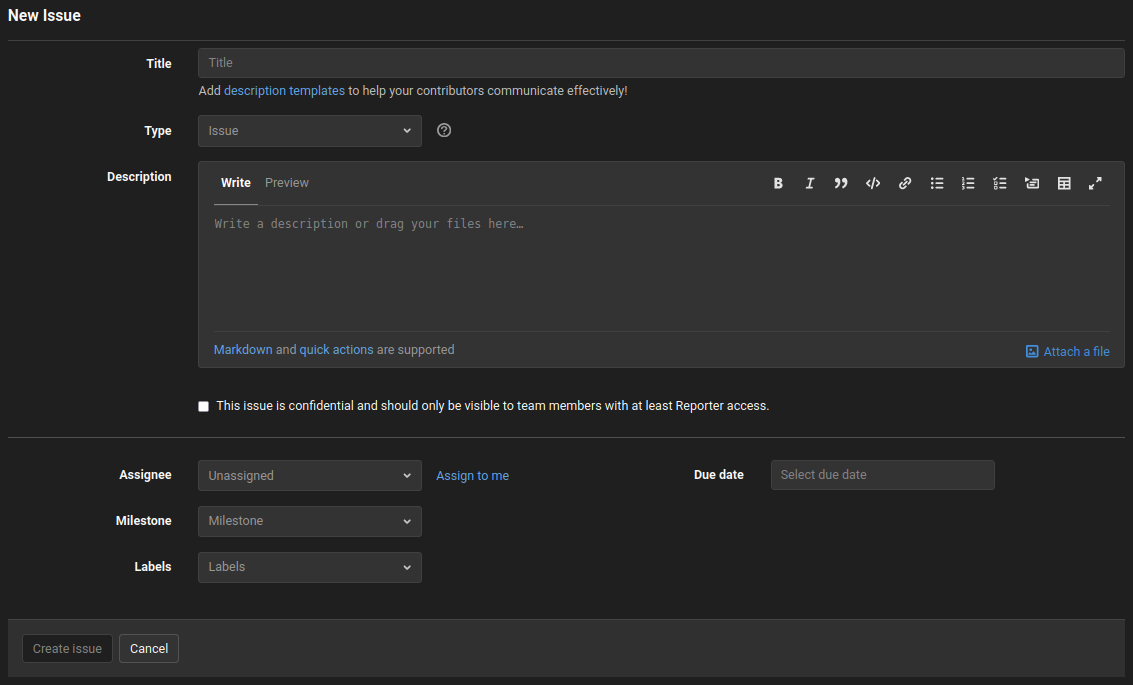
\includegraphics[width=105mm]{img/issue}};
      \node[inner sep=0pt, align=left] (txt) at (0.4,2.57) {\color{white} Short and comprehensible: "Implement password reset", "404 page", ...};
      \node[inner sep=0pt, align=left] (txt) at (-0.1,0.60) {\color{white} As short as possible, but may be quite long if necessary.\\ \color{white} Mention people with "@" (@user1), other issues with "\#" (\#138),\\ \color{white}other pull requests with "!" (!47), ...};
      \node[inner sep=0pt, align=left] (txt) at (0.7,-1.25) {\color{white} Tag the responsible for the issue (typically the one that will solve it, not the issue author)};
    \end{tikzpicture}
  \end{center}
\end{frame}

\begin{frame}[fragile]
\frametitle{2. Main subjects}
\framesubtitle{2.2. Branches}

A branch is an independent line of development. It allows people to develop in the same project in parallel, and to merge those changes at a later time

\vspace{0.5em}

\begin{minipage}{0.5\textwidth}
  \centering
  
  Branching

  \begin{lstlisting}[language=bash]
# go to master branch
git checkout master
# create feature branch from current commit/branch (master)
git checkout -b feature
  \end{lstlisting}

  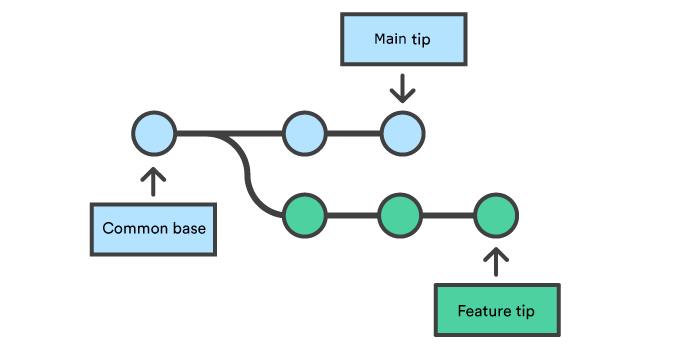
\includegraphics[height=30mm]{img/branch.png}
\end{minipage}%
\begin{minipage}{0.5\textwidth}
  \centering
  
  Merging

  \begin{lstlisting}[language=bash]
# go to master branch
git checkout master
# merge feature branch into master
git merge feature
  \end{lstlisting}
  
  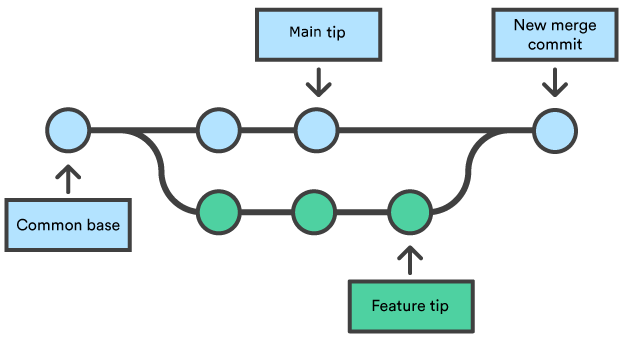
\includegraphics[height=30mm]{img/merge.png}
\end{minipage}%

\end{frame}
\begin{frame}
  \small

  There are many kinds of merges, but the ones we're interested in are the following between two branches:

  ~

\begin{minipage}[t]{0.49\textwidth}
  \footnotesize
  
  \begin{center}
    \includesvg[scale=0.3]{img/fast-forward-merge-2}
  \end{center}

  \textbf{Fast forward (2-way merge):} \texttt{master} has no new commits, and is forwarded to \texttt{feature}
  
\end{minipage}~~~
\begin{minipage}[t]{0.49\textwidth}
  \footnotesize

  \begin{center}
    \includesvg[scale=0.3]{img/three-way-merge-2}
  \end{center}

  \textbf{3-way merge:} \texttt{master} and \texttt{feature} have diverged at some point. git may be able to sort that out, \textbf{\color{red}or not}
  
\end{minipage}%

\end{frame}

\begin{frame}[fragile]
  \begin{minipage}{0.6\textwidth}
    \begin{itemize}
      \item 3-way merges are common, and git knows some automatic strategies that cover most 3-way merges.

      \item What is \textbf{not usual} is for git to struggle because \textbf{two people have made changes to the same part of the same file} in two different branches (\textit{merge conflict}), when they should not have.
      
      \begin{lstlisting}
<<<<<<< master
[...]
=======
[...]
>>>>>>> feature
      \end{lstlisting}

      \begin{itemize}
        \item Advise: don't use a pure editor to solve conflicts, or you're going to end up with forgotten \texttt{"<<<<<<<"} in your repo; use VS Code/GitHub Desktop/...
      \end{itemize}
      
    \end{itemize}
  \end{minipage}%
  \begin{minipage}{0.4\textwidth}
    \centering
    \includesvg[scale=0.25]{img/three-way-merge-2}
  \end{minipage}
\end{frame}

\begin{frame}
\frametitle{2. Main subjects}
\framesubtitle{2.3. Pull requests}

A \textit{pull request} (also \textit{merge request} in GitLab) is not a git feature; it is implemented by git hosts (GitHub/GitLab/...).

~

A pull request is a request that you make for your team members to review the feature you developed, or the fix you found for an issue.

~

Git hosts provide pull requests as spaces for developers to notify colleagues that they're done with a feature, and to discuss if that feature has issues or could be made in a different way.

\end{frame}

\begin{frame}
  \centering

  \tiny

  \begin{tikzpicture}
    \node[inner sep=0pt] (img) at (0,0) {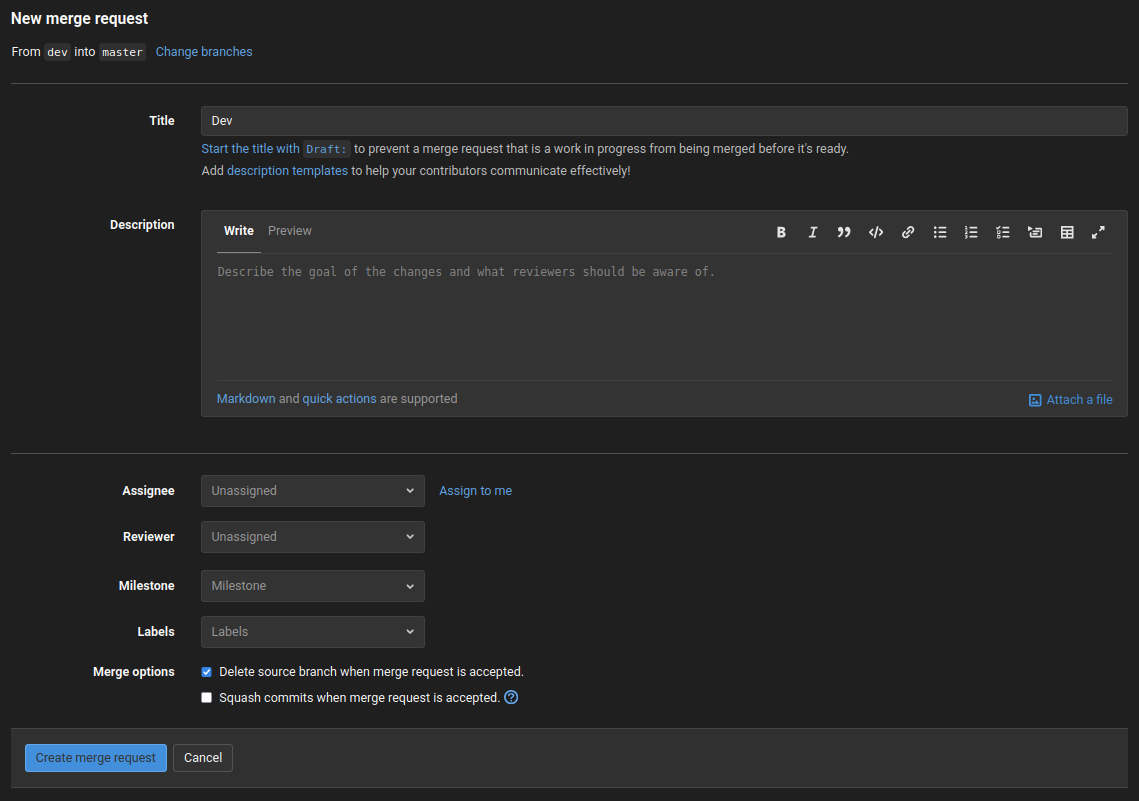
\includegraphics[width=120mm]{img/pr}};
    \node[inner sep=0pt, align=left] (txt) at (0.9,2.95) {\color{white} Short and comprehensible: "Fixes issue 138", "Implements password reset", "404 page", ...};
    % \draw [-stealth,color=white](-2,3.4) -- (-3,3);
    \node[inner sep=0pt, align=left] (txt) at (0.95,0.75) {\color{white} As short as possible, but may be quite long if necessary.\\ \color{white}If it fixes an issue, the issue should already contain info on the problem;\\ \color{white}you should primarily mention the solution (if the solution is self-explaining, you can leave it empty).\\ \color{white} Mention people with "@" (@user1), issues with "\#" (\#138), other pull requests with "!" (!47), ...};
    \node[inner sep=0pt, align=left] (txt) at (2.1,-0.95) {\color{white} Tag the responsible for the PR (typically the PR author)};
    \node[inner sep=0pt, align=left] (txt) at (0.6,-1.45) {\color{white} Specifically tag someone to review the PR};
    \node[inner sep=0pt, align=left] (txt) at (1.6,-2.85) {\color{white} Checked if you're done with that branch};
    \node[inner sep=0pt, align=left] (txt) at (1.25,-3.15) {\color{white} Leave this unchecked at all time};
  \end{tikzpicture}
\end{frame}

\begin{frame}
\frametitle{2. Main subjects}
\framesubtitle{2.4. Git Flow}

{\footnotesize (Actually I'll be talking about a simplification of Git Flow)}

~

\begin{itemize}
  \item A workflow is a set of rules that describes the steps a programmer should follow when developing/deploying

  \item git has a million possible workflows due to its flexibility, but there are some workflows that are better and more well-known than others

  \item \textbf{Git Flow} is a workflow based in branches.
\end{itemize}

\end{frame}

\begin{frame}
  \small

  Main rules:

  \begin{enumerate}
    \item \texttt{master} is the deployment branch (i.e., as bug-free as humanely possible).
    \item \texttt{dev} is the deployment branch; it stands between feature development and deployment. Should be relatively bug-free.
    \item Each feature/issue is developed in a different branch created from \texttt{dev}; the feature branch must have an explaining name (e.g., \texttt{page-404}, \texttt{issue/138}). When it is complete, merge it into \texttt{dev} and delete the feature branch.
  \end{enumerate}

  \begin{center}
    \includesvg[width=110mm]{img/gitflow}
  \end{center}
\end{frame}

\begin{frame}
  \small
  \begin{enumerate}
    
    \item When preparing a new release, create a new branch (e.g., \texttt{v1.0}). I don't usually do this, and you don't need to either, although it's part of Git Flow.
    \item To perform a \textit{hotfix}, 1. create new branch (typically using word \texttt{hotfix}) and fix the bug; 2. merge \texttt{hotfix} $\rightarrow$ \texttt{master}; 3. create a patch release from \texttt{master} (e.g, go from v1.2.3 to v1.2.4); 4. merge \texttt{hotfix} $\rightarrow$ \texttt{dev}; 5. delete \texttt{hotfix}
  \end{enumerate}

  \begin{center}
    \includesvg[width=110mm]{img/gitflow-2}
  \end{center}
\end{frame}

\begin{frame}
\frametitle{2. Main subjects}
\framesubtitle{2.5. GitHub Flow}

\scriptsize

Somewhat similar to Git Flow, but adding GitHub features:

\begin{enumerate}
  \item Each feature, bug and to-do item goes into an \textit{issue}
  \item Each merge goes first through code revision using a \textit{pull request}
  \item Issues and pull requests are visually tracked in a project board
\end{enumerate}

\begin{center}
  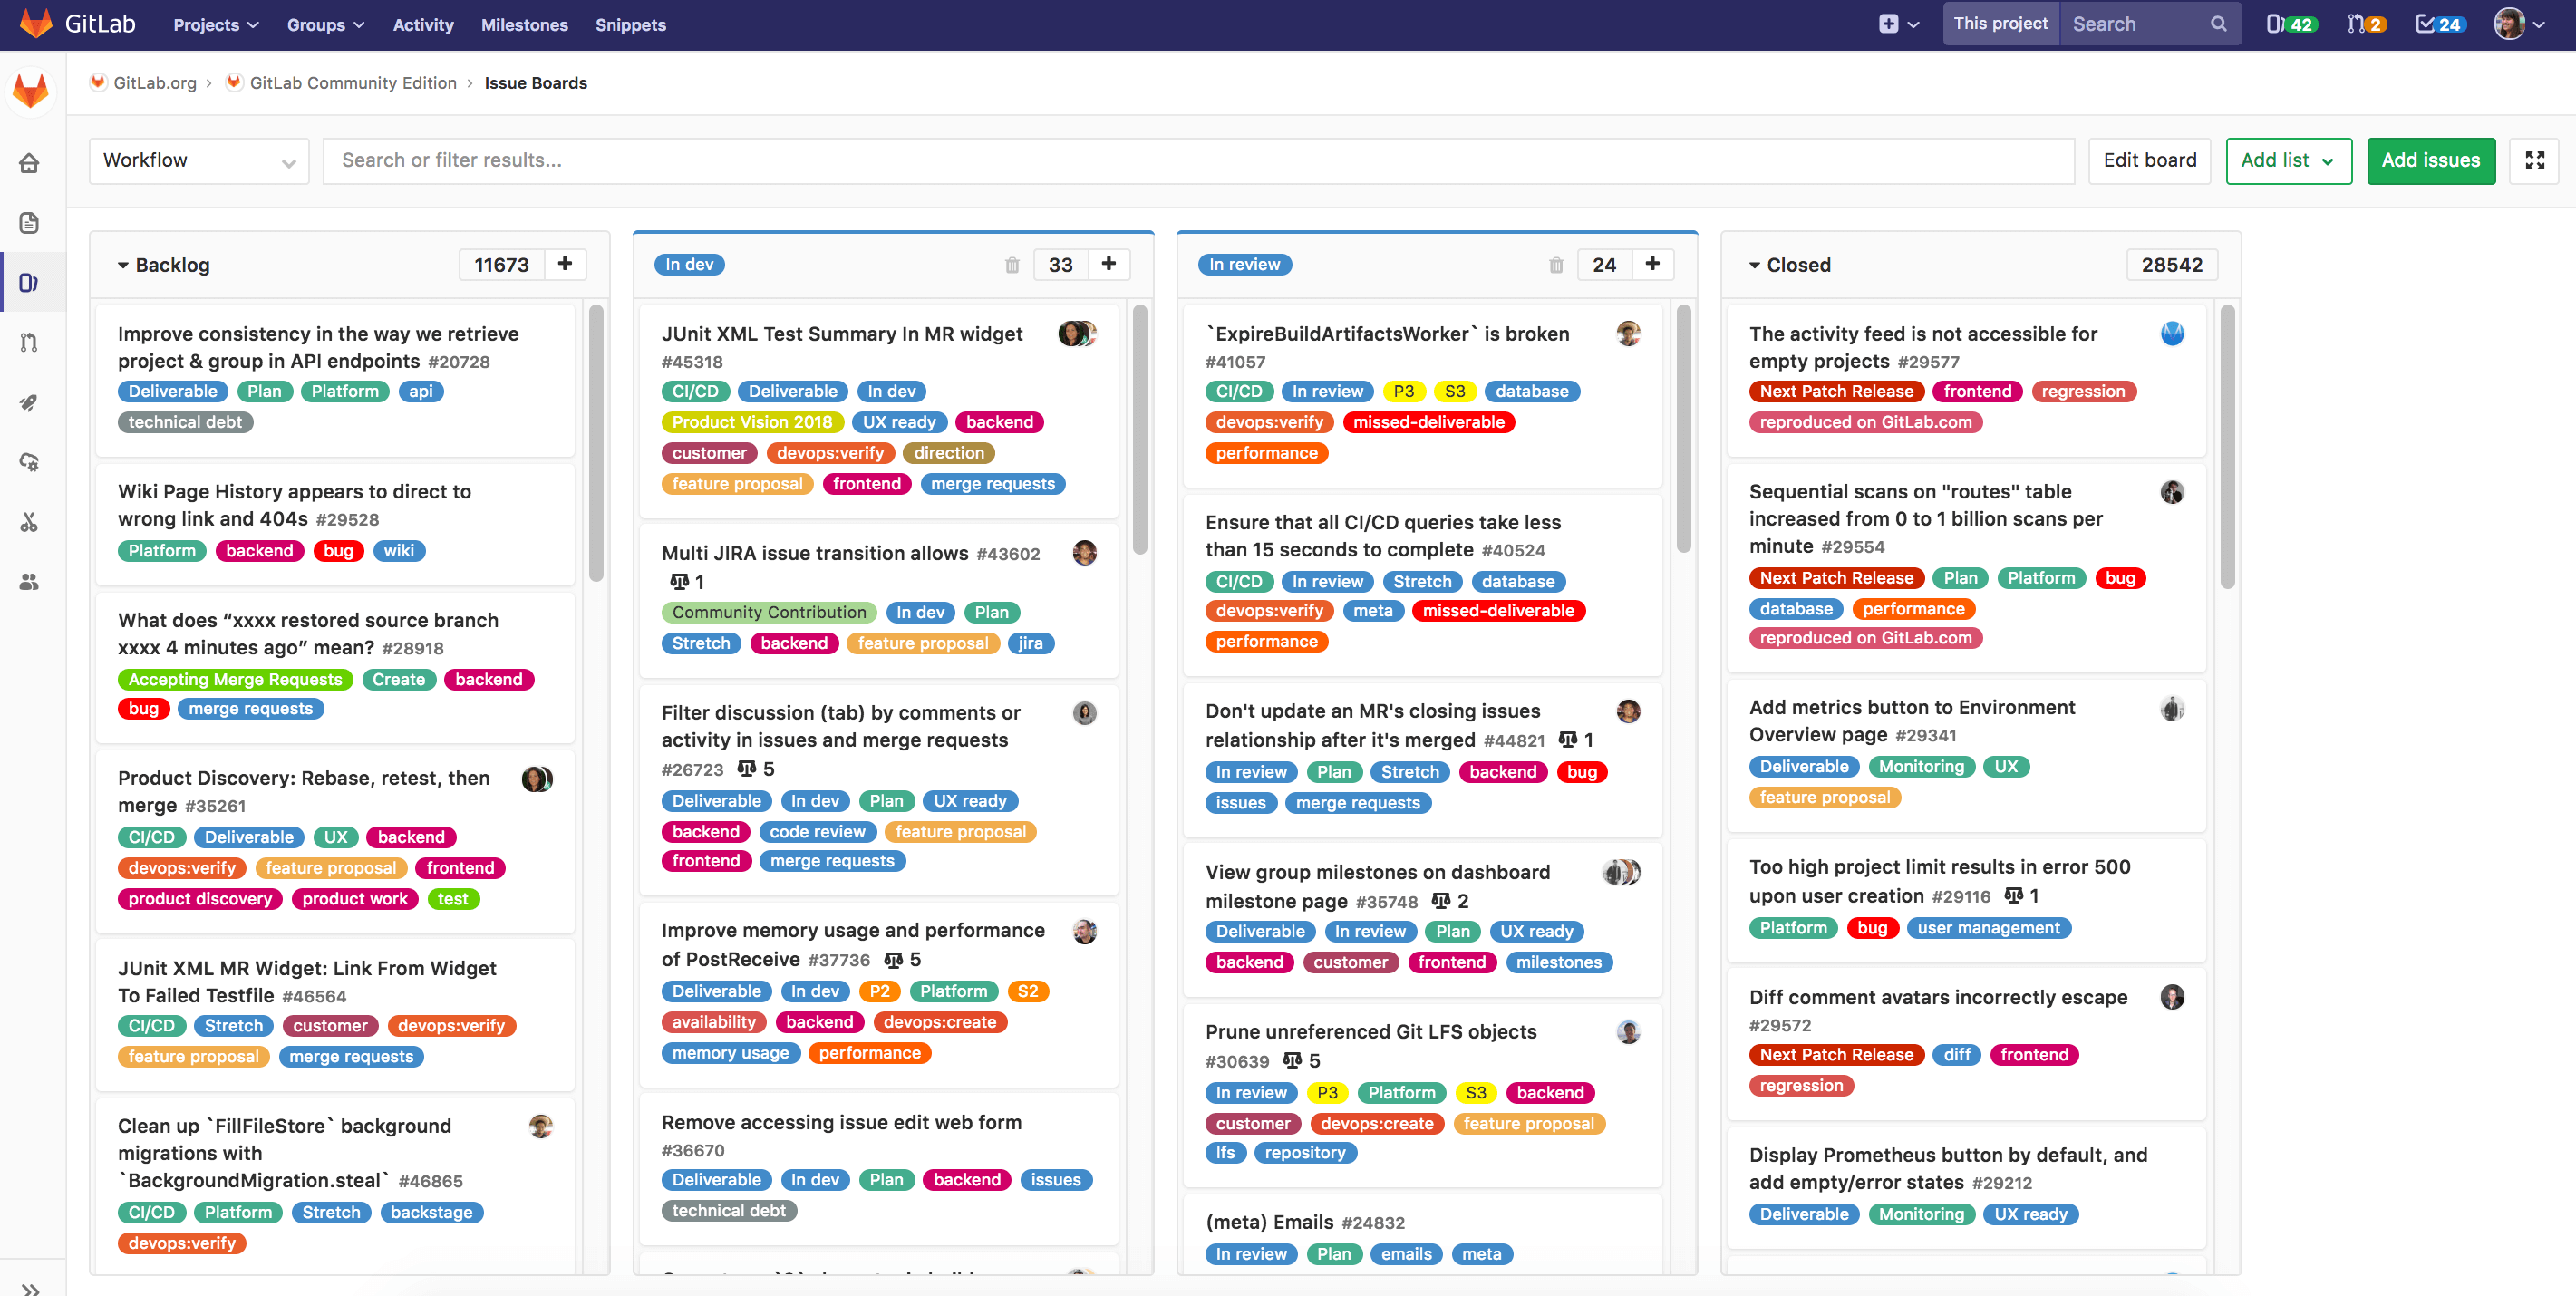
\includegraphics[width=110mm]{img/board}
\end{center}

\end{frame}

\begin{frame}
  \frametitle{References}
  \begin{enumerate}
    \item Git Branch | Atlassian Git Tutorial ({\footnotesize atlassian.com/git/tutorials/using-branches})
    \item Pull Requests | Atlassian Git Tutorial ({\footnotesize atlassian.com/git/tutorials/making-a-pull-request})
    \item Gitflow workflow | Atlassian Git Tutorial ({\footnotesize atlassian.com/git/tutorials/comparing-workflows/gitflow-workflow})
    \item 4 ways to use GitLab Issue Boards ({\footnotesize https://about.gitlab.com/blog/2018/08/02/4-ways-to-use-gitlab-issue-boards/})
  \end{enumerate}
\end{frame}

\end{document}
